\chapter{Estrategias de planificación de queries}
\label{cap:epq}

Decir por lotes

\section{Predicción de rendimiendo de transacciones de lectura}
\label{scheduling:prtl}
Conocer de antemano la eficiencia de una consulta es una ventaja importante para poder usar técnicas efectivas de planificación en motores de búsqueda. Por ejemplo, en el contexto de procesamiento paralelo de \textit{queries} por lotes (\textit{batches}) se pueden crear grupos de consultas que posean tiempos de respuesta parecidos, así se tiende a disminuir tanto el desbalance de carga entre los procesadores como el tiempo en procesar el \textit{batch} completo.
A continuación se presentan los métodos predictores implementados en el siguiente trabajo de tesis. 

\subsection{Método de predicción Glasgow}
\label{scheduling:glasgow}
El presente método \citep{Macdonald:2012} se basa en estadísticos obtenidos previamente calculados desde el índice invertido. Los puntajes de los documentos son obtenidos mediante el método BM25. Para cada consulta que llega al sistema, se toman los términos y para cada uno de ellos desde su propia lista invertida se obtiene los siguientes estadísticos $s(t)$:

\begin{list}{}{}
	\item \textbf{Media aritmética}. Se calcula la media aritmética del puntaje de los documentos.

	\item \textbf{Media geométrica}. Se calcula la media geométrica del puntaje de los documentos.

	\item \textbf{Media harmónica}.  Se calcula la media harmónica del puntaje de los documentos. 

	\item \textbf{Máximo puntaje}. Se obtiene el puntaje máximo perteneciente a algún documento dentro de la lista invertida. En otras palabras, se obtiene el \textit{upper bound} $UB_t$ de la lista. 

	\item \textbf{Varianza del puntaje}. Se extrae la varianza de puntaje de los documentos desde la lista invertida del término $t$. 
	
	\item \textbf{Número de documentos}. Se calcula el largo de la lista invertida. 

	\item \textbf{Número de maximos}. Se obtiene el número de veces en que aparece un puntaje máximo, es decir, el número de veces en que se actualiza el puntaje máximo. 

	\item \textbf{Número de documentos mayor a la media}. Se extrae el número de documentos que sobrepasa en puntaje al puntaje promedio. 
	
	\item \textbf{Número de documentos con puntaje máximo}. Se calcula el número de documentos que tienen el puntaje máximo dentro en la lista invertida del término $t$. 
	
	\item \textbf{Número de documentos dentro del 5\% más alto}. Se obtiene el número de documentos cuyos puntajes están dentro del 5\% superior dentrl de la lista invertida. 
	
	\item \textbf{Número de documentos dentro del 5\% del umbral (\textit{threshold})}. Se calcula el número de documentos cuyos puntaje están dentro del 5\% superior o inferior al umbral. Recordar que el \textit{threshold} es el puntaje de documento más bajo dentro del conjunto de los \textit{top-K}.
	
	\item \textbf{Número de inserciones en el conjunto de los mejores K documentos}. Para obtener este estadístico se asume que el término $t$ es una consulta con un solo término, se resuelve esta \textit{query} con el método \textit{Wand}  y se calcula el número de inserciones de documentos que se hizo al \textit{heap}. Recordar que las inserciones al \textit{heap} ocurren cuando el puntaje aproximado del documento supera el puntaje más bajo que en el \textit{heap} en ese momento (umbral o \textit{threshold}).
	
	\item \textbf{Frecuencia inversa de documento del término}. Se calcula el \textit{idf} del término $t$.
	
	\item \textbf{Tiempo en ser procesado el término}. Se obtiene el tiempo que toma ser procesado el término como una \textit{query} de un solo término.

\end{list}


Cada uno de los 14 estadísticos mencionados anteriormente están relacionados linealmente con la eficiencia de una transacción de lectura y son la base para la implementación del predictor, que está basado en un modelo de regresión lineal múltiple \citep{Chambers:1991}. A continuacion se muestra un resumen de estos estadísitcos en la Tabla \ref{tabla:estadisticosGlasgow}. 

\begin{table}[H]
\centering
\caption{Resumen de los estadísticos que se deben extraer desde el índice invertido}
\label{tabla:estadisticosGlasgow}
\begin{tabular}{|l|}
	\hline
	\textbf{Estadísticos del término s(t)} \\	
	1. Media aritmética	 \\ \hline
	2. Media geométrica	 \\ \hline
	3. Media harmónica	 \\ \hline
	4. Máximo puntaje	 \\ \hline
	5. Varianza del puntaje	 \\ \hline
	6. Número de documentos	 \\ \hline
	7. Número de máximos	 \\ \hline
	8. Número docs > media	 \\ \hline
	9. Número docs = máximo puntaje	 \\ \hline
	10. Número docs dentro del 5\% más alto	 \\ \hline
	11. Número docs dentro del 5\% del umbral	 \\ \hline
	12. Número de incerciones al conjunto top-K	 \\ \hline
	13. IDF	 \\ \hline
	14. Tiempo en resolver $t$ como \textit{query}	\\ \hline  
\end{tabular}
\end{table}


\subsection{Método de predicción SIGIR}
\label{scheduling:sigir}
Aquí va la explicación del método de SIGIR 2014


\section{Wand \textit{multi-threaded}}
\label{scheduling:wm}
Dado que el método WAND \citep{Broder:2003} consiste es el método del estado del arte ocupado hoy en día por los motores de búsqueda, en esta investigación se asume un sistema que usa este método para obtener eficientemente los mejores K documentos a una transacción de lectura. Este algoritmo usa un \textit{ranking} basado en una evaluación de dos niveles. En el primer nivel, este usa una cota superior (\textit{upper bound}) al puntaje de cada documento para intentar descartarlos eficientemente. En el segundo nivel se computa el puntaje real de los documentos que pasa el primer nivel. Se utiliza una estructura de datos llamada \textit{heap} que va guardando el conjunto de los mejores K documentos hasta un determinado instante. El menor puntaje de este conjunto es usado como umbral (\textit{threshold}) para las evaluaciones del primer nivel, de esta forma se descarta rápidamente documentos que no pueden ser parte del conjunto final de los \textit{top-K} documentos. Esto permite un eficiente y a la vez seguro proceso de descarte que asegura que en el resultado final se encontrará el conjunto correcto y no se perderán documentos relevantes.

Existen dos formas de implementar WAND \textit{multithreaded}. Una de ellas es usando \textit{heaps} locales (LH), es decir, un \textit{heap} por hilo de ejecución (\textit{thread}) y el otro es usando \textit{heaps} compartidos (SH). El estudio en \citep{Rojas:2013} se muestra indicios que el esquema SH es generalmente más eficiente. Logrando rápidamente un óptimo valor para el threshold, el esquema SH posee las siguientes ventajas: (1) Se puede reducir el número de calculo de puntajes completos y (2) se ejecutan pocas operaciones de actualización del heap (reduciendo el número de \textit{locks} que se hace a la estructura de dato). A continuación se presenta el diseño llevado a cabo para ambos esquemas.


\subsection{Wand con heaps locales}
En el esquema LH, cada \textit{thread} procesa una porción del índice invertido mientras mantiene un \textit{heap} local con los mejores $K$ documentos que el específico hilo de ejecución ha encontrado hasta ahora. Al final del proceso, los resultados deben ser reunido en un solo conjunto final global. Los resultados en \citep{Rojas:2013} muestran que el esquema LH es más eficientes para aquellas transacciones que toman poco tiempo en ser resueltas. En la Figura \ref{fig:wand-heap-local} se muestra el esquema de ejecución para \textit{heaps} locales explicado anteriormente. 

\begin{figure}[!ht]
\centering
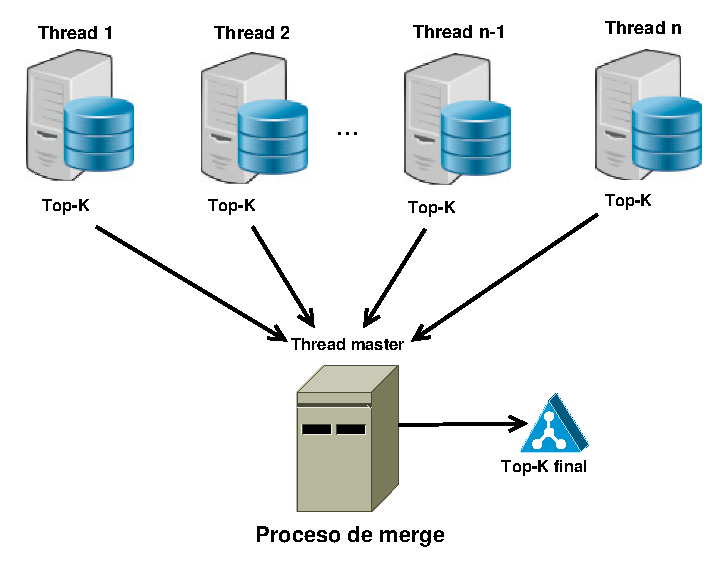
\includegraphics[scale=.75]{images/wand_heaps_locales.eps}
\caption{Esquema de ejecución de algoritmo WAND con heaps locales}
\label{fig:wand-heap-local}
\end{figure}

El diseño aplicado para implementar el esquema LH se puede ver en la Figura \ref{fig:TopKMultiThreadWandOperatorLocal}. La clase principal es la TopKMultiThreadWandOperatorLocal, que es la encargada de controlar el paralelismo en la resolución de las transacciones. Para explicar de mejor manera cada una de las clases involucradas en la implementación, se presenta el siguiente diccionario de datos.

\begin{sidewaysfigure}[!ht]
\centering
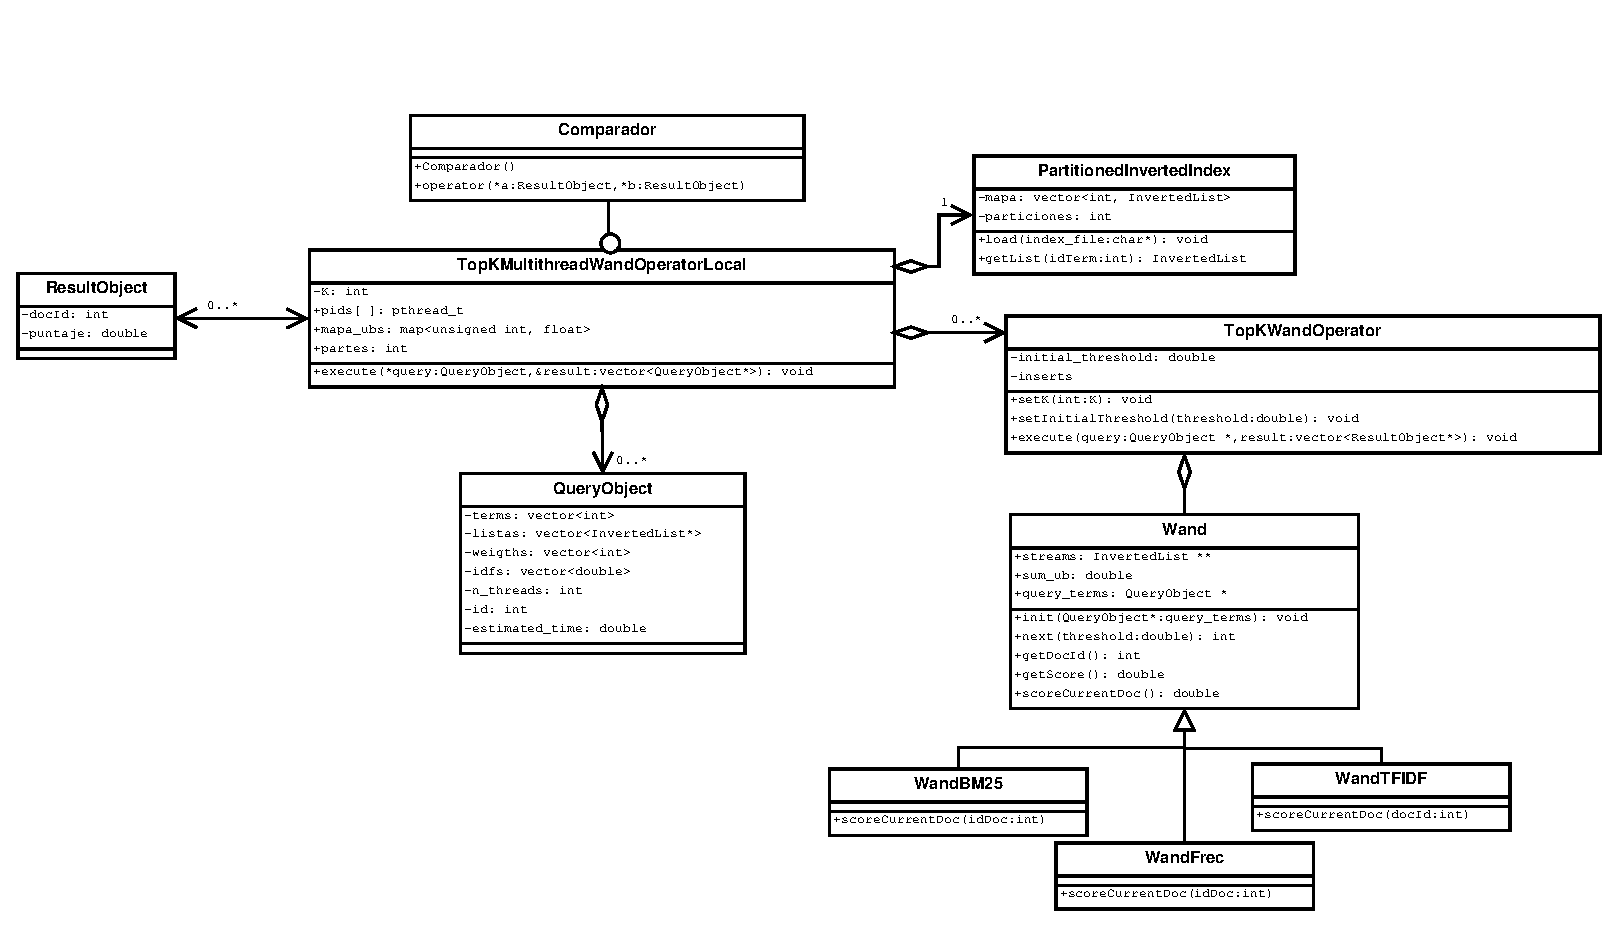
\includegraphics[scale=.75]{images/TopKMultiThreadWandOperatorLocal.eps}
\caption{Diagrama de clases para el esquema LH}
\label{fig:TopKMultiThreadWandOperatorLocal}
\end{sidewaysfigure}

\begin{list}{}{}
	\item \textbf{TopKMultiThreadWandOperatorLocal}. Clase encargada de devolver los mejores K documentos para una query dada. Si es que la query debe ser resuelta en forma paralela, esta clase además debe controlar el paralelismo que se produce en la resolución de ésta, inicializando las variables correspondientes para lanzar los hilos de ejecución y luego escogiendo los mejores documentos desde todos los heaps creados por los diferentes threads (proceso de merge). En esta clase se define un mapa que asocia cada término del índice invertido con el puntaje del mejor documento en esa lista invertida (upper bound de la lista invertida) y además se define cuántos documentos se van a retornar al final del proceso (atributo K). El método execute inicializa las variables locales para los diferentes threads, posteriormente hace el llamado al método \emph{thread-execute} (en el cual se llevará a cabo la resolución de la transacción de lectura en forma paralela), finalmente se toman los resultados parciales de cada uno de los hilos de ejecución y se ejecuta el proceso que mezcla los resultados, retornando solo los mejores K documentos. 
	
	\item \textbf{PartitionedInvertedIndex}. Clase que tiene la tarea de almacenar el índice invertido y extraer desde aquí las listas invertidas de documentos para cada uno de los términos de las transacciones de lectura. El almacenamiento el índice se lleva a cabo mediante un mapa cada término su lista invertida correspondiente y para la extracción de estas listas se usa el método getList.
	
	\item \textbf{TopKWandOperator}.  Cada thread tendrá su propio objeto TopKWandOperator encargado de obtener los mejores K documentos. El cálculo de este conjunto se realiza en el método execute con la ayuda de un objeto de tipo Wand asociado.
	
	\item \textbf{Wand}. Clase que controla la lógica del algoritmo wand. Lleva a cabo el proceso de inserción de documentos en el heap y todo lo que esto conlleva. Existen diferentes tipos de objetos Wand que se pueden utilizar, entre ellos están WandBM25, WandFrec y WandTFIDF, donde la única diferencia entre ellos es el método de que calcula el puntaje de cada documento. Por ejemplo, WandBM25 utiliza BM25 (citar) y WandTFIDF utiliza tf-idf (citar también). 
	
	\item \textbf{ResultObject}. Clase que se utiliza para guardar los mejores K documentos.
	
	\item \textbf{QueryObject}. Clase que representa una transacción de lectura. Está constutuída sus términos,  las respectivas listas invertidas y pesos de cada uno de ellos, la cantidad de threads con los cuales se resolverá dicha transacción y el tiempo estimado de procesamiento (este tiempo se predice al momento de resolver la query).

\end{list}




\subsection{Wand con heap compartido}
\label{scheduling:whc}
En el esquema SH cada thread procesa una porción del índice. Sin embargo, ahora un solo heap es creado y accedido por todos los threads. En este caso no se requiere de mezclar los resultados y el proceso de descarte tiende a ser más eficiente porque los documentos con mayor puntaje tienden a estar en el heap. Acceder al heap debe ser controlado por un lock o algún método similar que garantice el acceso exclusivo de los threads al heap. Este esquema es más eficiente que el LH en queries que toman mayor tiempo en ser resueltas.

El diseño implementado para este esquema posee como clase principal a TopKMultiThreadWandOperatorLocks y difiere del modelo implementado para el esquema LH en el sentido que ahora se debe controlar el acceso concurrente a los datos compartidos como el heap y el threshold. A continuación se presenta el diccionario de datos del esquema SH mostrado en la Figura \ref{fig:TopKMultiThreadWandOperatorLocks}.

\begin{figure}[!ht]
\centering
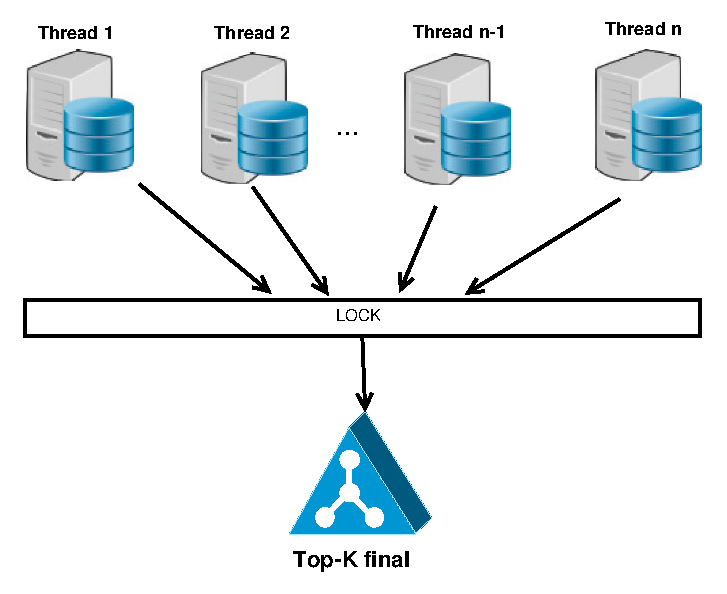
\includegraphics[scale=.75]{images/wand_heaps_compartido.eps}
\caption{Esquema de ejecución de algoritmo WAND con heap compartido}
\label{fig:wand-heap-compartido}
\end{figure}

\begin{list}{}{}
	\item \textbf{TopKMultiThreadWandOperatorLocks}. Clase encargada de inicializar las variables compartidas y de lanzar los threads requeridos para procesar la transacción de lectura.
	
	\item \textbf{WandThreadData}. Clase anidada a TopKMultiThreadWandOperatorLocks que contendrá todas las variables compartidas para el procesamiento de las consultas. Dentro de los atributos más importantes destaca el mutex utilizado para controlar el acceso al heap compartido y además al threshold (en este esquema es un threshold global y compartido a todos los threads).
	
	\item \textbf{Wand}. Al igual que en el esquema anterior, esta clase se encarga de llevar a cabo el proceso de inserción de documentos en el heap y de las actualizaciones del threshold. El método scoreCurrentDoc es el encargado de entregarle un puntaje a cada documento y dependerá de qué tipo de Wand se este utilizando (BM25, WandFrec, WandTFIDF). 

	\item \textbf{PartitionedInvertedIndex}. Clase encargada de almacenar el índice invertido. Posee un método llamado getList que recibe como parámetro el identificador de un documento y retorna la lista invertida asociada. 

\end{list}

\begin{sidewaysfigure}[!ht]
\centering
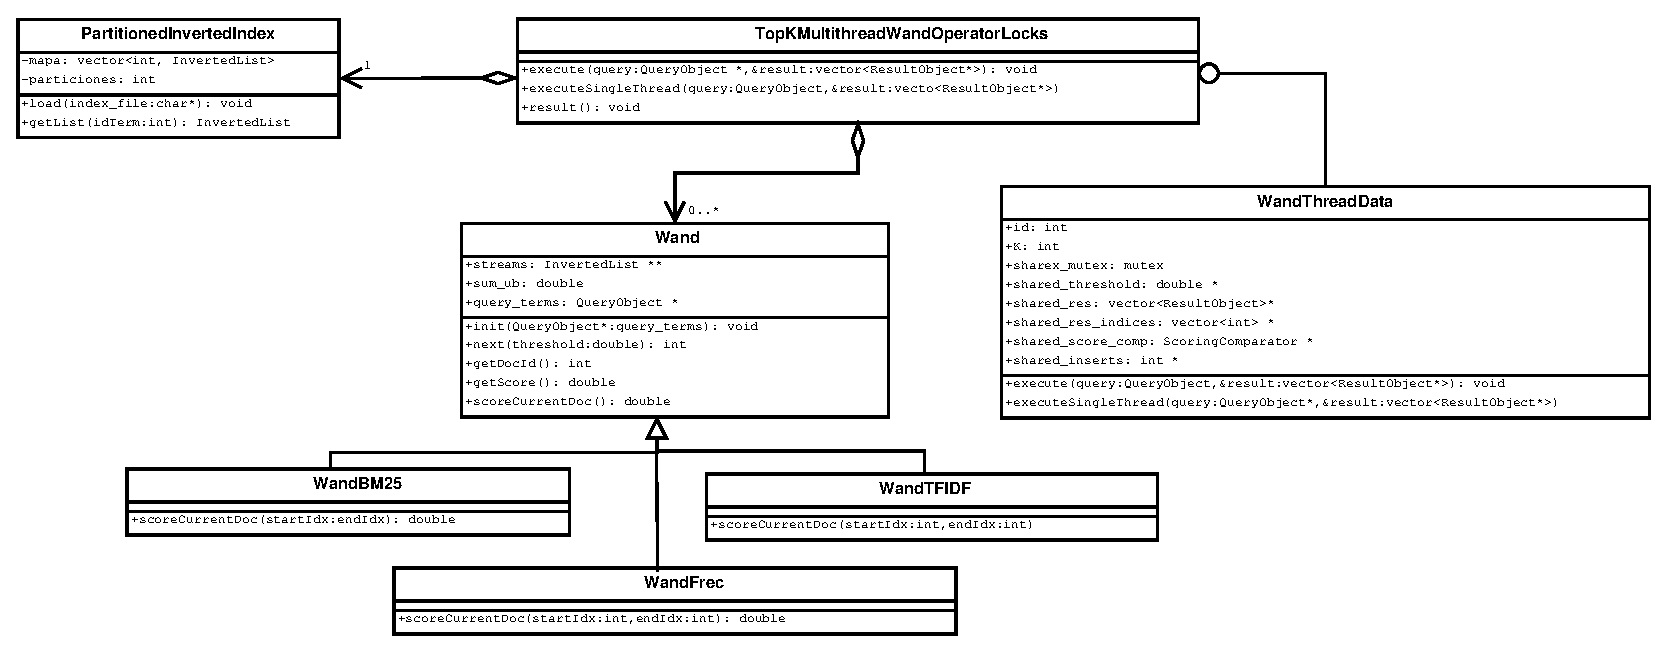
\includegraphics[scale=.75]{images/TopKMultiThreadWandOperatorLocks.eps}
\caption{Diagrama de clases para el esquema SH}
\label{fig:TopKMultiThreadWandOperatorLocks}
\end{sidewaysfigure}


\section{Estrategia \textit{baseline}}
\label{scheduling:baseline}
Un simple camino para construir un sistema que responda a múltiples consultas simultáneamente usando múltiple hilos de ejecución, es usando estos hilos de manera independiente. Para hacer esto se debe mantener un conjunto de \textit{threads} consumidores que trabajarán en paralelo y se encargarán de resolver las \textit{queries} secuencialmente (una a una) desde una misma cola, esto es lo que en este trabajo se denomina estrategia de Un Thread Por Query (1TQ). En la Figura \ref{fig:1TQ} se puede apreciar el esquema de ejecución en donde cada uno de los procesos genera una petición de alguna consulta en la cola, si quedan \textit{queries} por procesar entonces se le asigna al proceso una consulta que tendrá que resolver de manera secuencial. Se debe tener en cuenta que cada vez que un proceso genera una solicitud de \textit{query}, se bloquea la estructura de datos que contiene las consultas a procesar y luego se procesa la solicitud, de esta forma se asegura un acceso seguro por parte de los distintos \textit{threads}. 

\begin{figure}[H]
\centering
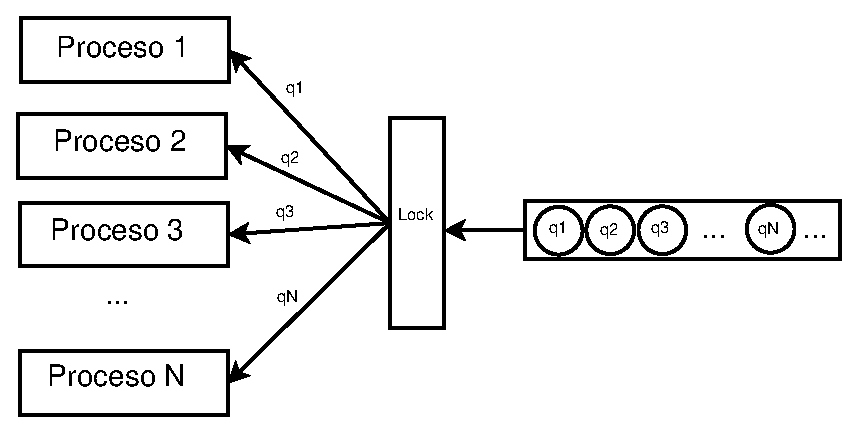
\includegraphics[scale=.75]{images/1TQ.eps}
\caption{Ejemplo de procesamiento estrategia 1TQ}
\label{fig:1TQ}
\end{figure}

Este esquema tiene la ventaja que es simple y fácil de implementar y controlar. Sin embargo, existen sistemas de recuperación de la información como los motores de búsqueda verticales que cuando están ejecutando \textit{batches} de \textit{queries} deben parar su ejecución porque transacciones de escritura han llegado al sistema, y este deben actualizar la información del índice invertido. Solo después de la fase de actualización el sistema es capaz de ejecutar el siguiente \textit{batch} de transacciones de lectura. Al final de cada conjunto de consultas, es posible que algunos hilos de ejecución del sistema finalicen su trabajo y que no tengan más \textit{queries} para procesar, por lo que ellos tienen que esperar que los \textit{threads} restantes finalicen su trabajo antes que el sistema entre en la fase de actualización de su índice invertido o bien, se pase a la ejecución del siguiente \textit{batch} de consultas.
Sin embargo, aunque cada hilo de ejecución está secuencialmente ejecutando una transacción de lectura diferente, algunas de estas operaciones puede tomar un tiempo cosiderable, de esta forma se produce una importante pérdida de eficiencia, aunque la intuición nos dice que esto se puede mitigar con \textit{queries} que requieran poca cantidad de tiempo para ser procesada (trabajos pequeños o \textit{small jobs}). 
En la Figura \ref{fig:small_jobs} queda reflejado lo dicho en el párrafo anterior. Si los trabajos que cada \textit{thread} está ejecutando son pequeños, entonces probablemente la pérdida de trabajo al final de cada \textit{batch} de consultas será menor al trabajo que se pierde cuando los trabajos son grandes (ver Figura \ref{fig:large_jobs}).  


\begin{figure}[H]
\centering
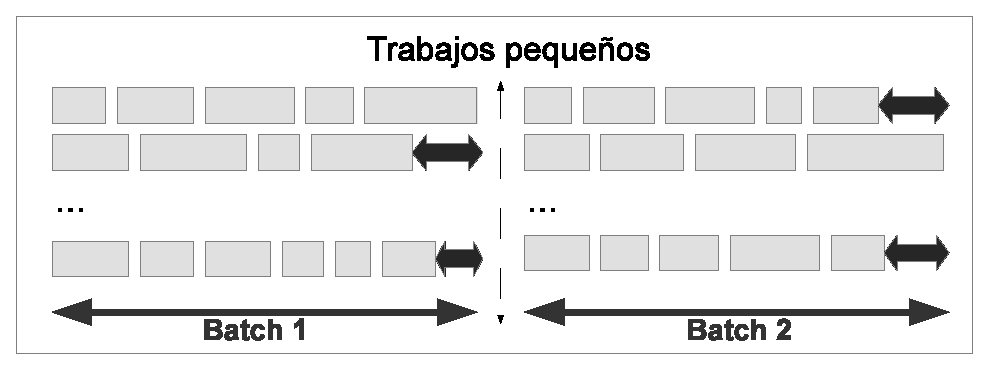
\includegraphics[scale=.75]{images/small_jobs.eps}
\caption{Ejecución en paralelo de \textit{small jobs}}
\label{fig:small_jobs}
\end{figure}

\begin{figure}[H]
\centering
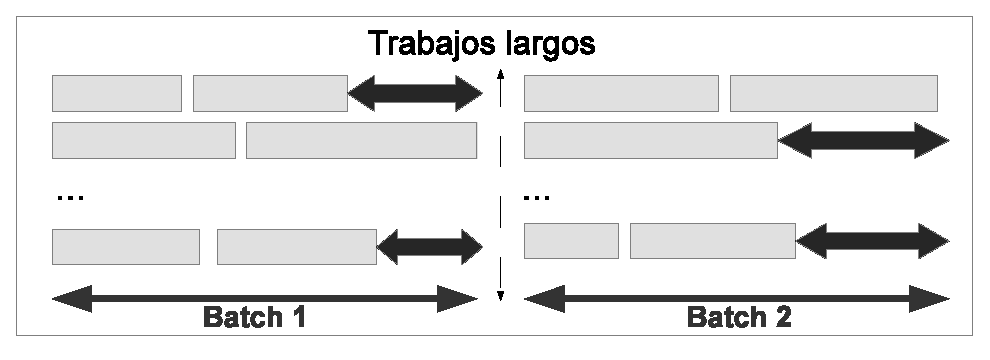
\includegraphics[scale=.75]{images/large_jobs.eps}
\caption{Ejecución en paralelo de \textit{large jobs}}
\label{fig:large_jobs}
\end{figure}


\section{Estrategias de \textit{scheuling}}
\label{scheduling:es}
nosotros optamos por un enfoque de Wand Heap Compartido para ser usado en los experimentos.
\subsection{FR}
\label{scheduling:fr}

\subsection{Times}
\label{scheduling:times}

\subsection{TimesRanges}
\label{scheduling:timesranges}




\section{Estrategia de unidades de trabajo}
\label{scheduling:unidadestrabajo}